\chapter{Design}\label{ch:design}
Nu hvor der både er taget højde for de informationer og funktioner der skal være i systemet, kan der nu laves interaktions- og designklassediagram. De vil blive designet på baggrund af diagrammerne fra Analyse afsnittet og trelagsarktitekturen. 

\section{Kommunikationsdiagram}
Kommunikationsdiagrammet viser de centrale trin fra Use Casen automatisk lagerstyring, som også er vist i SSD på figur \ref{fig:ssd}. Kommunikationsdiagrammet bruges for at vise hvilke klasser der laver metodekald og hvor de kald fører hen.

\begin{landscape}
    \begin{figure}[p]
        \centering
        \includegraphics[width=\hsize]{figures/design/Kommunikationsdiagram}
        \caption{Kommunikationsdiagram}
        \label{fig:Kommunikationsdiagram}
    \end{figure}
\end{landscape}
\todo{write more stuff about diagram}

\section{Designklassediagram}
Designklassediagrammet er det tætteste vi kommer på en præcis repræsentation af programmet. Den viser samtlige klasser, metoder, attributter og relationer, så det blot er kildekoden der skal implementeres. Designklassediagrammet giver også et godt overblik arkitekturen af programmet, og Designklassediagrammet skulle gerne reflektere domænemodellen, og Kommunikationsdiagrammet.

\begin{landscape}
    \begin{figure}
        \centering
        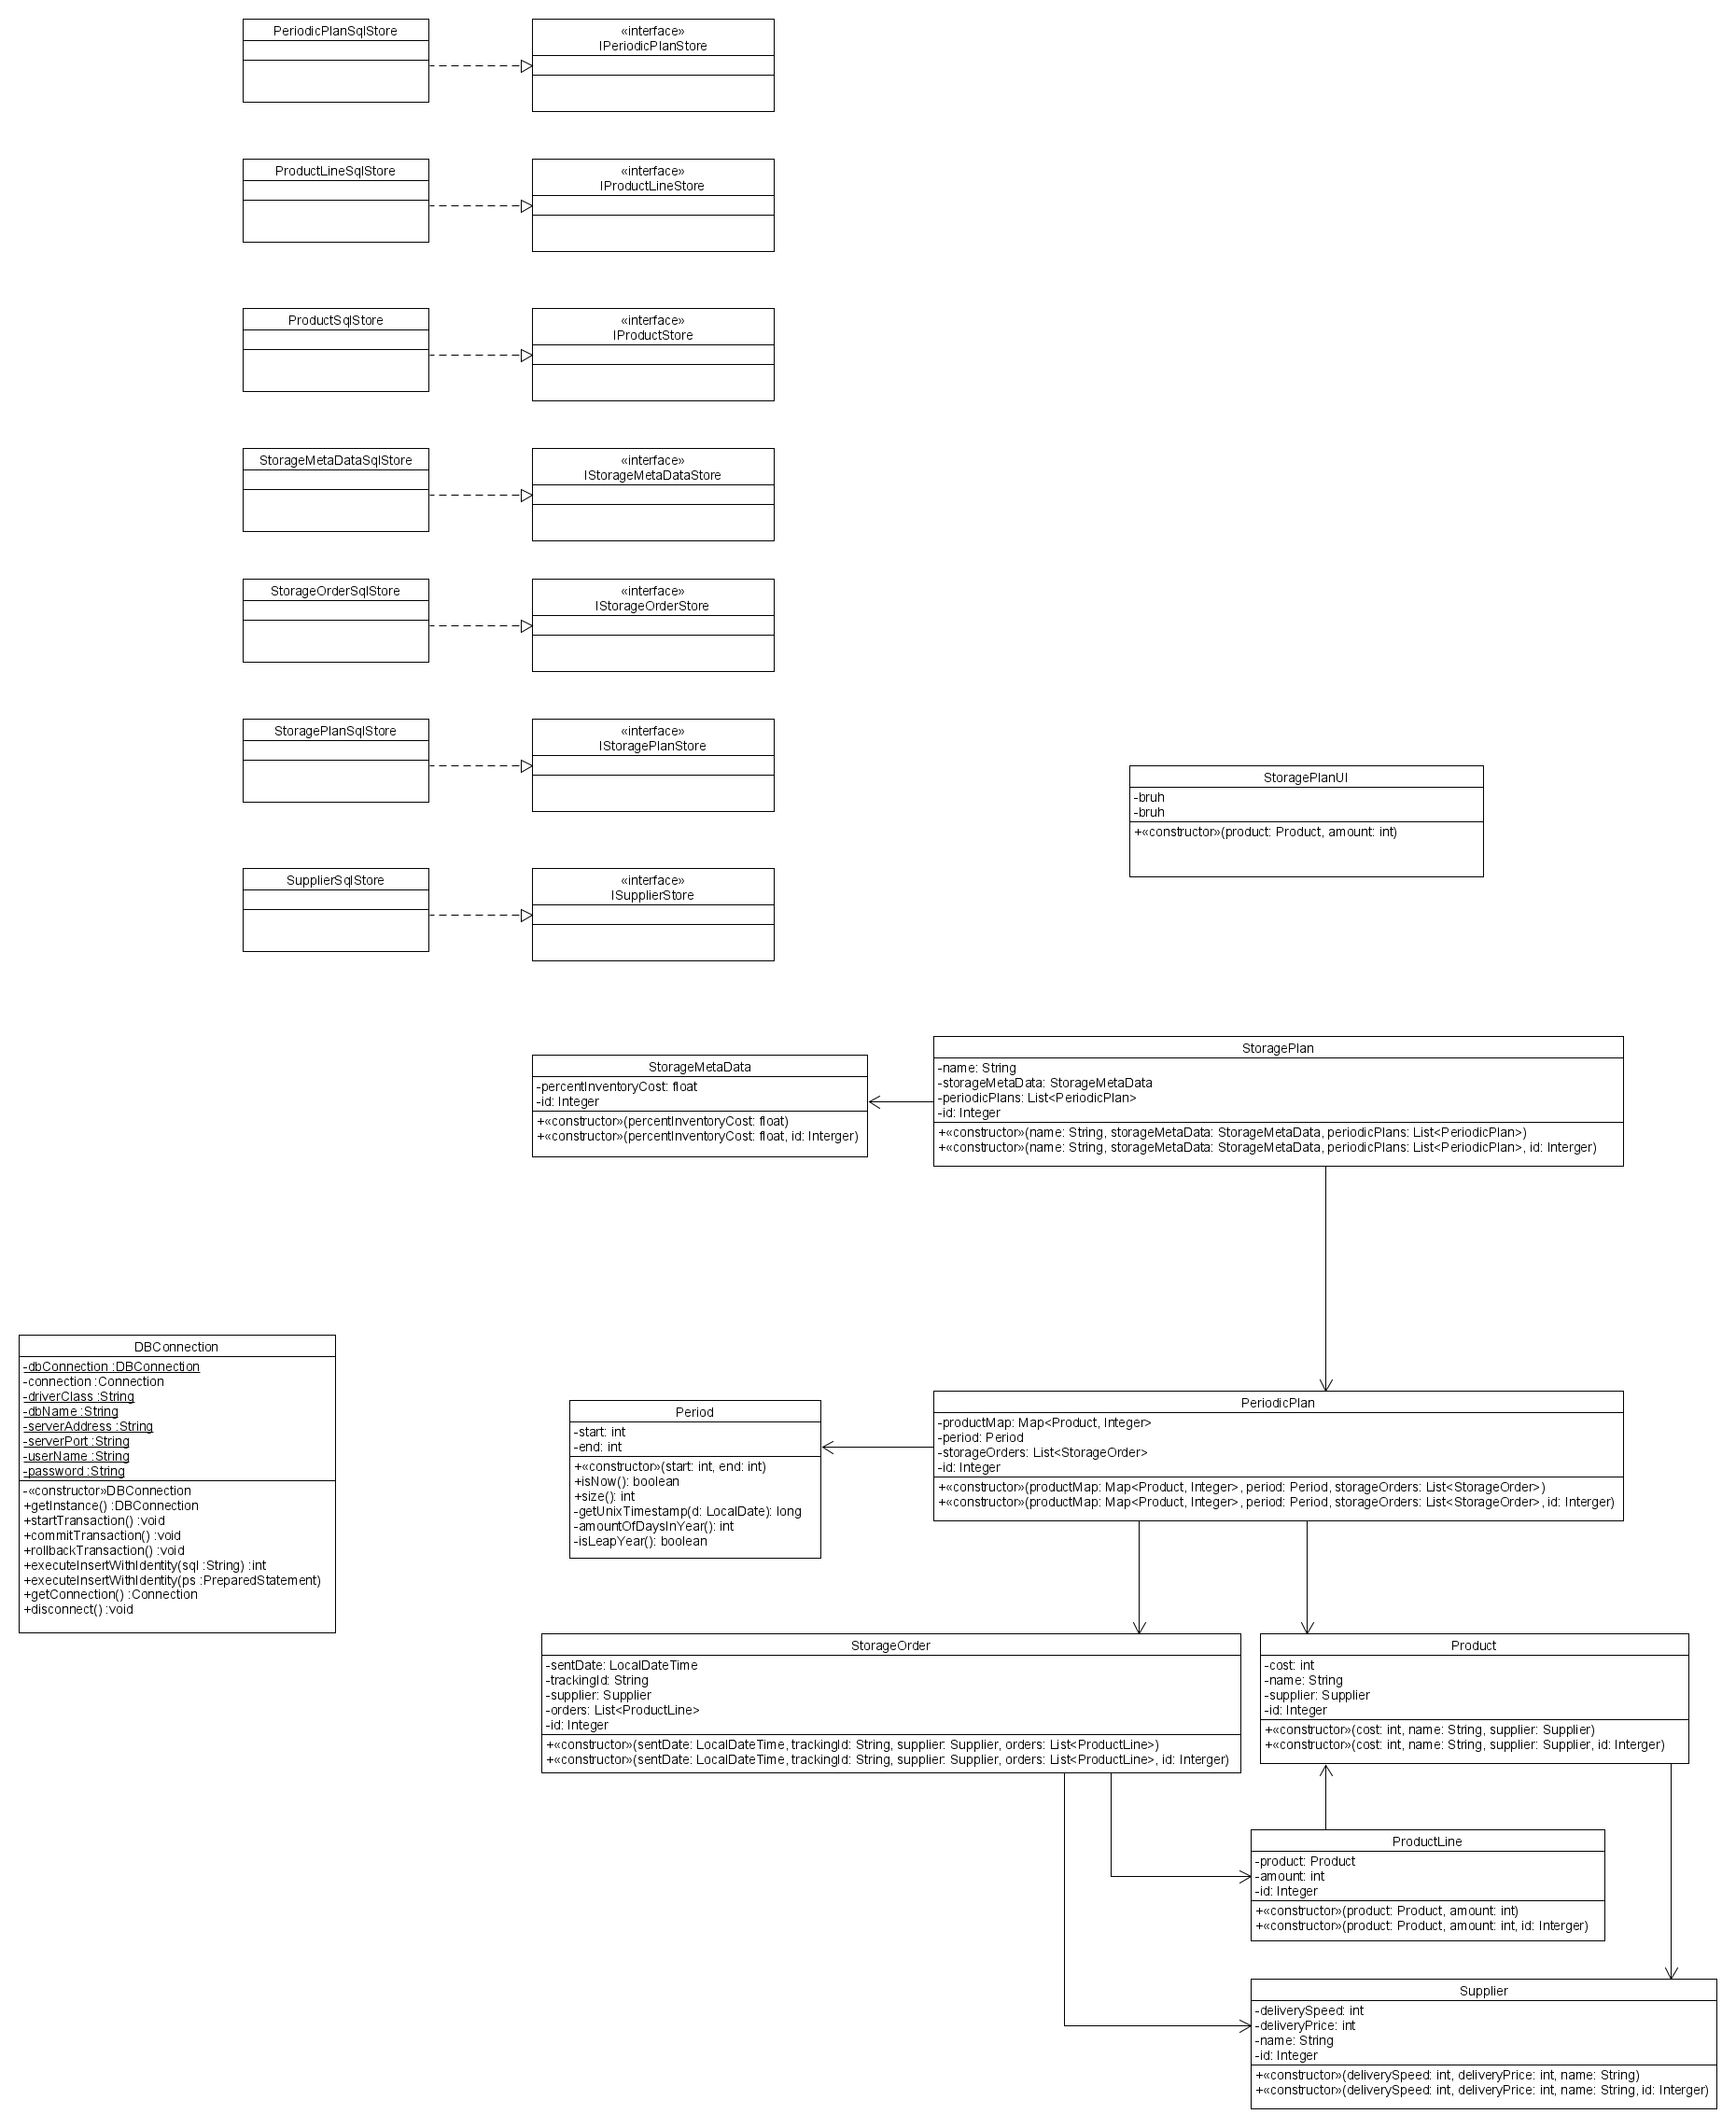
\includegraphics[width=0.6\hsize]{figures/design/designclassdiagram}
        \caption{Designklassediagram}
        \label{fig:new_designclassdiagram}
    \end{figure}
\end{landscape}
\todo{write more stuff about architecture and "smart" ideas}
Som det kan ses er der brugt en afslappet lagdelt arkitektur, hvori der indgår et UI lag, et controller lag, et model-og-database lag\cite{Larman2004}. UI laget er brugergrænsefladen og tillader brugeren at interagere med programmet. Controller laget håndterer informationsændringer mv. og er de centrale komponenter til at udføre en Use Case. Model-og-database laget indeholder de klasser, der fremgik i domænemodellen \ref{fig:domain_model_2}, deres attributter og metoder - i database-delen sørges der for persistens og organisering af data. 
For at kunne gennemføre en god lagdelt struktur, kræves der forskellige design mønstre. Det kan ses at DBConnection er en Singleton mønster\cite{Larman2004}, som sørger for at der kun oprettes én instans af DBConnection. DBConnection benyttes af alle \verb|SqlStore| klasserne for at kunne gemme data i databasen. Udover det ses det også, at der er benyttet et DAO mønster\cite{DAO} med alle Controller klasser. Dette ses ud fra at all controllers har en interface til database operationer, og ved forholdet til modelklasserne.
%superclass pattern